% Options for packages loaded elsewhere
\PassOptionsToPackage{unicode}{hyperref}
\PassOptionsToPackage{hyphens}{url}
%
\documentclass[
]{book}
\usepackage{amsmath,amssymb}
\usepackage{lmodern}
\usepackage{ifxetex,ifluatex}
\ifnum 0\ifxetex 1\fi\ifluatex 1\fi=0 % if pdftex
  \usepackage[T1]{fontenc}
  \usepackage[utf8]{inputenc}
  \usepackage{textcomp} % provide euro and other symbols
\else % if luatex or xetex
  \usepackage{unicode-math}
  \defaultfontfeatures{Scale=MatchLowercase}
  \defaultfontfeatures[\rmfamily]{Ligatures=TeX,Scale=1}
\fi
% Use upquote if available, for straight quotes in verbatim environments
\IfFileExists{upquote.sty}{\usepackage{upquote}}{}
\IfFileExists{microtype.sty}{% use microtype if available
  \usepackage[]{microtype}
  \UseMicrotypeSet[protrusion]{basicmath} % disable protrusion for tt fonts
}{}
\makeatletter
\@ifundefined{KOMAClassName}{% if non-KOMA class
  \IfFileExists{parskip.sty}{%
    \usepackage{parskip}
  }{% else
    \setlength{\parindent}{0pt}
    \setlength{\parskip}{6pt plus 2pt minus 1pt}}
}{% if KOMA class
  \KOMAoptions{parskip=half}}
\makeatother
\usepackage{xcolor}
\IfFileExists{xurl.sty}{\usepackage{xurl}}{} % add URL line breaks if available
\IfFileExists{bookmark.sty}{\usepackage{bookmark}}{\usepackage{hyperref}}
\hypersetup{
  pdftitle={A Minimal Book Example},
  pdfauthor={Yihui Xie},
  hidelinks,
  pdfcreator={LaTeX via pandoc}}
\urlstyle{same} % disable monospaced font for URLs
\usepackage{color}
\usepackage{fancyvrb}
\newcommand{\VerbBar}{|}
\newcommand{\VERB}{\Verb[commandchars=\\\{\}]}
\DefineVerbatimEnvironment{Highlighting}{Verbatim}{commandchars=\\\{\}}
% Add ',fontsize=\small' for more characters per line
\usepackage{framed}
\definecolor{shadecolor}{RGB}{248,248,248}
\newenvironment{Shaded}{\begin{snugshade}}{\end{snugshade}}
\newcommand{\AlertTok}[1]{\textcolor[rgb]{0.94,0.16,0.16}{#1}}
\newcommand{\AnnotationTok}[1]{\textcolor[rgb]{0.56,0.35,0.01}{\textbf{\textit{#1}}}}
\newcommand{\AttributeTok}[1]{\textcolor[rgb]{0.77,0.63,0.00}{#1}}
\newcommand{\BaseNTok}[1]{\textcolor[rgb]{0.00,0.00,0.81}{#1}}
\newcommand{\BuiltInTok}[1]{#1}
\newcommand{\CharTok}[1]{\textcolor[rgb]{0.31,0.60,0.02}{#1}}
\newcommand{\CommentTok}[1]{\textcolor[rgb]{0.56,0.35,0.01}{\textit{#1}}}
\newcommand{\CommentVarTok}[1]{\textcolor[rgb]{0.56,0.35,0.01}{\textbf{\textit{#1}}}}
\newcommand{\ConstantTok}[1]{\textcolor[rgb]{0.00,0.00,0.00}{#1}}
\newcommand{\ControlFlowTok}[1]{\textcolor[rgb]{0.13,0.29,0.53}{\textbf{#1}}}
\newcommand{\DataTypeTok}[1]{\textcolor[rgb]{0.13,0.29,0.53}{#1}}
\newcommand{\DecValTok}[1]{\textcolor[rgb]{0.00,0.00,0.81}{#1}}
\newcommand{\DocumentationTok}[1]{\textcolor[rgb]{0.56,0.35,0.01}{\textbf{\textit{#1}}}}
\newcommand{\ErrorTok}[1]{\textcolor[rgb]{0.64,0.00,0.00}{\textbf{#1}}}
\newcommand{\ExtensionTok}[1]{#1}
\newcommand{\FloatTok}[1]{\textcolor[rgb]{0.00,0.00,0.81}{#1}}
\newcommand{\FunctionTok}[1]{\textcolor[rgb]{0.00,0.00,0.00}{#1}}
\newcommand{\ImportTok}[1]{#1}
\newcommand{\InformationTok}[1]{\textcolor[rgb]{0.56,0.35,0.01}{\textbf{\textit{#1}}}}
\newcommand{\KeywordTok}[1]{\textcolor[rgb]{0.13,0.29,0.53}{\textbf{#1}}}
\newcommand{\NormalTok}[1]{#1}
\newcommand{\OperatorTok}[1]{\textcolor[rgb]{0.81,0.36,0.00}{\textbf{#1}}}
\newcommand{\OtherTok}[1]{\textcolor[rgb]{0.56,0.35,0.01}{#1}}
\newcommand{\PreprocessorTok}[1]{\textcolor[rgb]{0.56,0.35,0.01}{\textit{#1}}}
\newcommand{\RegionMarkerTok}[1]{#1}
\newcommand{\SpecialCharTok}[1]{\textcolor[rgb]{0.00,0.00,0.00}{#1}}
\newcommand{\SpecialStringTok}[1]{\textcolor[rgb]{0.31,0.60,0.02}{#1}}
\newcommand{\StringTok}[1]{\textcolor[rgb]{0.31,0.60,0.02}{#1}}
\newcommand{\VariableTok}[1]{\textcolor[rgb]{0.00,0.00,0.00}{#1}}
\newcommand{\VerbatimStringTok}[1]{\textcolor[rgb]{0.31,0.60,0.02}{#1}}
\newcommand{\WarningTok}[1]{\textcolor[rgb]{0.56,0.35,0.01}{\textbf{\textit{#1}}}}
\usepackage{longtable,booktabs,array}
\usepackage{calc} % for calculating minipage widths
% Correct order of tables after \paragraph or \subparagraph
\usepackage{etoolbox}
\makeatletter
\patchcmd\longtable{\par}{\if@noskipsec\mbox{}\fi\par}{}{}
\makeatother
% Allow footnotes in longtable head/foot
\IfFileExists{footnotehyper.sty}{\usepackage{footnotehyper}}{\usepackage{footnote}}
\makesavenoteenv{longtable}
\usepackage{graphicx}
\makeatletter
\def\maxwidth{\ifdim\Gin@nat@width>\linewidth\linewidth\else\Gin@nat@width\fi}
\def\maxheight{\ifdim\Gin@nat@height>\textheight\textheight\else\Gin@nat@height\fi}
\makeatother
% Scale images if necessary, so that they will not overflow the page
% margins by default, and it is still possible to overwrite the defaults
% using explicit options in \includegraphics[width, height, ...]{}
\setkeys{Gin}{width=\maxwidth,height=\maxheight,keepaspectratio}
% Set default figure placement to htbp
\makeatletter
\def\fps@figure{htbp}
\makeatother
\setlength{\emergencystretch}{3em} % prevent overfull lines
\providecommand{\tightlist}{%
  \setlength{\itemsep}{0pt}\setlength{\parskip}{0pt}}
\setcounter{secnumdepth}{5}
\usepackage{booktabs}
\usepackage{amsthm}
\makeatletter
\def\thm@space@setup{%
  \thm@preskip=8pt plus 2pt minus 4pt
  \thm@postskip=\thm@preskip
}
\makeatother
\ifluatex
  \usepackage{selnolig}  % disable illegal ligatures
\fi
\usepackage[]{natbib}
\bibliographystyle{apalike}

\title{A Minimal Book Example}
\author{Yihui Xie}
\date{2022-03-11}

\begin{document}
\maketitle

{
\setcounter{tocdepth}{1}
\tableofcontents
}
\hypertarget{prerequisites}{%
\chapter{Prerequisites}\label{prerequisites}}

This is a \emph{sample} book written in \textbf{Markdown}. You can use anything that Pandoc's Markdown supports, e.g., a math equation \(a^2 + b^2 = c^2\).

The \textbf{bookdown} package can be installed from CRAN or Github:

\begin{Shaded}
\begin{Highlighting}[]
\FunctionTok{install.packages}\NormalTok{(}\StringTok{"bookdown"}\NormalTok{)}
\CommentTok{\# or the development version}
\CommentTok{\# devtools::install\_github("rstudio/bookdown")}
\end{Highlighting}
\end{Shaded}

Remember each Rmd file contains one and only one chapter, and a chapter is defined by the first-level heading \texttt{\#}.

To compile this example to PDF, you need XeLaTeX. You are recommended to install TinyTeX (which includes XeLaTeX): \url{https://yihui.name/tinytex/}.

\hypertarget{intro}{%
\chapter{Introduction}\label{intro}}

You can label chapter and section titles using \texttt{\{\#label\}} after them, e.g., we can reference Chapter \ref{intro}. If you do not manually label them, there will be automatic labels anyway, e.g., Chapter \ref{methods}.

Figures and tables with captions will be placed in \texttt{figure} and \texttt{table} environments, respectively.

\begin{Shaded}
\begin{Highlighting}[]
\FunctionTok{par}\NormalTok{(}\AttributeTok{mar =} \FunctionTok{c}\NormalTok{(}\DecValTok{4}\NormalTok{, }\DecValTok{4}\NormalTok{, .}\DecValTok{1}\NormalTok{, .}\DecValTok{1}\NormalTok{))}
\FunctionTok{plot}\NormalTok{(pressure, }\AttributeTok{type =} \StringTok{\textquotesingle{}b\textquotesingle{}}\NormalTok{, }\AttributeTok{pch =} \DecValTok{19}\NormalTok{)}
\end{Highlighting}
\end{Shaded}

\begin{figure}

{\centering \includegraphics[width=0.8\linewidth]{bookdown-demo_files/figure-latex/nice-fig-1} 

}

\caption{Here is a nice figure!}\label{fig:nice-fig}
\end{figure}

Reference a figure by its code chunk label with the \texttt{fig:} prefix, e.g., see Figure \ref{fig:nice-fig}. Similarly, you can reference tables generated from \texttt{knitr::kable()}, e.g., see Table \ref{tab:nice-tab}.

\begin{Shaded}
\begin{Highlighting}[]
\NormalTok{knitr}\SpecialCharTok{::}\FunctionTok{kable}\NormalTok{(}
  \FunctionTok{head}\NormalTok{(iris, }\DecValTok{20}\NormalTok{), }\AttributeTok{caption =} \StringTok{\textquotesingle{}Here is a nice table!\textquotesingle{}}\NormalTok{,}
  \AttributeTok{booktabs =} \ConstantTok{TRUE}
\NormalTok{)}
\end{Highlighting}
\end{Shaded}

\begin{table}

\caption{\label{tab:nice-tab}Here is a nice table!}
\centering
\begin{tabular}[t]{rrrrl}
\toprule
Sepal.Length & Sepal.Width & Petal.Length & Petal.Width & Species\\
\midrule
5.1 & 3.5 & 1.4 & 0.2 & setosa\\
4.9 & 3.0 & 1.4 & 0.2 & setosa\\
4.7 & 3.2 & 1.3 & 0.2 & setosa\\
4.6 & 3.1 & 1.5 & 0.2 & setosa\\
5.0 & 3.6 & 1.4 & 0.2 & setosa\\
\addlinespace
5.4 & 3.9 & 1.7 & 0.4 & setosa\\
4.6 & 3.4 & 1.4 & 0.3 & setosa\\
5.0 & 3.4 & 1.5 & 0.2 & setosa\\
4.4 & 2.9 & 1.4 & 0.2 & setosa\\
4.9 & 3.1 & 1.5 & 0.1 & setosa\\
\addlinespace
5.4 & 3.7 & 1.5 & 0.2 & setosa\\
4.8 & 3.4 & 1.6 & 0.2 & setosa\\
4.8 & 3.0 & 1.4 & 0.1 & setosa\\
4.3 & 3.0 & 1.1 & 0.1 & setosa\\
5.8 & 4.0 & 1.2 & 0.2 & setosa\\
\addlinespace
5.7 & 4.4 & 1.5 & 0.4 & setosa\\
5.4 & 3.9 & 1.3 & 0.4 & setosa\\
5.1 & 3.5 & 1.4 & 0.3 & setosa\\
5.7 & 3.8 & 1.7 & 0.3 & setosa\\
5.1 & 3.8 & 1.5 & 0.3 & setosa\\
\bottomrule
\end{tabular}
\end{table}

You can write citations, too. For example, we are using the \textbf{bookdown} package \citep{R-bookdown} in this sample book, which was built on top of R Markdown and \textbf{knitr} \citep{xie2015}.

\hypertarget{literature}{%
\chapter{Literature}\label{literature}}

Here is a review of existing methods.

\hypertarget{assignment-3-snow-data}{%
\chapter{Assignment 3 : Snow Data}\label{assignment-3-snow-data}}

\hypertarget{overview}{%
\section{Overview}\label{overview}}

Understanding the seasonal delivery and distribution of mountain snow cover, snowpack, and seasonal trends is important to the American West and to snowmelt-watered regions everywhere.The Center for Snow and Avalanche Studies established and operates the Senator Beck Basin Study Area as a purpose-built mountain system observatory in an alpine headwater catchment of the Uncompahgre River at Red Mountain Pass, in the western San Juan Mountains of southwest Colorado. Senator Beck Basin is located in a critically wet and cold portion of the Colorado River Basin.

Here is a map from the Center for Snow and Avalanche Studies indicating sample site locations in Colorado, USA (\url{http://snowstudies.org/sbbsa1.html}). The Senator Beck Study Plot (SBSP), Swamp Angel Study Plot (SASP), and associated Senator Beck Stream Gauge (SBSG) and Putney Study Plot (PTSP) are indicated by yellow triangles within the Senator Beck Basin (SBB).

\includegraphics{https://snowstudies.org/Area_AirPhoto_wLocation_650w.png}
In the assignment below, I'll work through manipulating some of the precipitation and temperature data collected as part of the long term Mountain System Monitoring.

\hypertarget{methods}{%
\section{Methods}\label{methods}}

This analysis uses the \texttt{SASP\ forcing} and \texttt{SBSP\_forcing} meteorological data sets to understand how temperature and precipitation patterns change with time at the two sites.

\hypertarget{analysis-and-discussion}{%
\section{Analysis and Discussion}\label{analysis-and-discussion}}

\hypertarget{q1-extract-the-meteorological-data-urls.-here-we-want-you-to-use-the-rvest-package-to-get-the-urls-for-the-sasp-forcing-and-sbsp_forcing-meteorological-datasets.}{%
\subsection{\texorpdfstring{Q1: Extract the meteorological data URLs. Here we want you to use the \texttt{rvest} package to get the URLs for the \texttt{SASP\ forcing} and \texttt{SBSP\_forcing} meteorological datasets.}{Q1: Extract the meteorological data URLs. Here we want you to use the rvest package to get the URLs for the SASP forcing and SBSP\_forcing meteorological datasets.}}\label{q1-extract-the-meteorological-data-urls.-here-we-want-you-to-use-the-rvest-package-to-get-the-urls-for-the-sasp-forcing-and-sbsp_forcing-meteorological-datasets.}}

\begin{Shaded}
\begin{Highlighting}[]
\NormalTok{site\_url }\OtherTok{\textless{}{-}} \StringTok{\textquotesingle{}https://snowstudies.org/archived{-}data/\textquotesingle{}}

\CommentTok{\#Read the web url}
\NormalTok{webpage }\OtherTok{\textless{}{-}} \FunctionTok{read\_html}\NormalTok{(site\_url)}

\CommentTok{\#Extract only weblinks and then the URLs!}
\NormalTok{links }\OtherTok{\textless{}{-}}\NormalTok{ webpage }\SpecialCharTok{\%\textgreater{}\%}
  \FunctionTok{html\_nodes}\NormalTok{(}\StringTok{\textquotesingle{}a\textquotesingle{}}\NormalTok{) }\SpecialCharTok{\%\textgreater{}\%} \CommentTok{\#a indicates a link to something }
\NormalTok{  .[}\FunctionTok{grepl}\NormalTok{(}\StringTok{\textquotesingle{}forcing\textquotesingle{}}\NormalTok{,.)] }\SpecialCharTok{\%\textgreater{}\%}
  \FunctionTok{html\_attr}\NormalTok{(}\StringTok{\textquotesingle{}href\textquotesingle{}}\NormalTok{)}
\NormalTok{links}
\end{Highlighting}
\end{Shaded}

\begin{verbatim}
## [1] "https://snowstudies.org/wp-content/uploads/2022/02/SBB_SASP_Forcing_Data.txt"
## [2] "https://snowstudies.org/wp-content/uploads/2022/02/SBB_SBSP_Forcing_Data.txt"
\end{verbatim}

\hypertarget{q2-download-the-meteorological-data.-use-the-download_file-and-str_split_fixed-commands-to-download-the-data-and-save-it-in-your-data-folder.}{%
\section{\texorpdfstring{Q2: Download the meteorological data. Use the \texttt{download\_file} and \texttt{str\_split\_fixed} commands to download the data and save it in your data folder.}{Q2: Download the meteorological data. Use the download\_file and str\_split\_fixed commands to download the data and save it in your data folder.}}\label{q2-download-the-meteorological-data.-use-the-download_file-and-str_split_fixed-commands-to-download-the-data-and-save-it-in-your-data-folder.}}

Downloaded data in a for loop

\begin{Shaded}
\begin{Highlighting}[]
\CommentTok{\#Grab only the name of the file by splitting out on forward slashes}
\NormalTok{splits }\OtherTok{\textless{}{-}} \FunctionTok{str\_split\_fixed}\NormalTok{(links,}\StringTok{\textquotesingle{}/\textquotesingle{}}\NormalTok{,}\DecValTok{8}\NormalTok{)}
\NormalTok{splits}
\end{Highlighting}
\end{Shaded}

\begin{verbatim}
##      [,1]     [,2] [,3]              [,4]         [,5]      [,6]   [,7]
## [1,] "https:" ""   "snowstudies.org" "wp-content" "uploads" "2022" "02"
## [2,] "https:" ""   "snowstudies.org" "wp-content" "uploads" "2022" "02"
##      [,8]                       
## [1,] "SBB_SASP_Forcing_Data.txt"
## [2,] "SBB_SBSP_Forcing_Data.txt"
\end{verbatim}

\begin{Shaded}
\begin{Highlighting}[]
\CommentTok{\#Keep only the 8th column}
\NormalTok{dataset }\OtherTok{\textless{}{-}}\NormalTok{ splits[,}\DecValTok{8}\NormalTok{] }\SpecialCharTok{\%\textgreater{}\%}
  \FunctionTok{gsub}\NormalTok{(}\StringTok{\textquotesingle{}.txt\textquotesingle{}}\NormalTok{,}\StringTok{\textquotesingle{}\textquotesingle{}}\NormalTok{,.)}

\CommentTok{\#generate a file list for where the data goes}
\NormalTok{file\_names }\OtherTok{\textless{}{-}} \FunctionTok{paste0}\NormalTok{(}\StringTok{\textquotesingle{}data/\textquotesingle{}}\NormalTok{,dataset)}
\NormalTok{datapath }\OtherTok{=} \StringTok{\textquotesingle{}data/\textquotesingle{}}
\FunctionTok{dir.create}\NormalTok{(datapath)}
\NormalTok{file\_names }\OtherTok{\textless{}{-}} \FunctionTok{paste0}\NormalTok{(datapath,dataset)}

\ControlFlowTok{for}\NormalTok{(i }\ControlFlowTok{in} \DecValTok{1}\SpecialCharTok{:}\DecValTok{2}\NormalTok{)\{}
  \FunctionTok{download.file}\NormalTok{(links[i],}\AttributeTok{destfile=}\NormalTok{file\_names[i])}
\NormalTok{\}}

\NormalTok{downloaded }\OtherTok{\textless{}{-}} \FunctionTok{file.exists}\NormalTok{(file\_names)}

\NormalTok{evaluate }\OtherTok{\textless{}{-}} \SpecialCharTok{!}\FunctionTok{all}\NormalTok{(downloaded)}
\end{Highlighting}
\end{Shaded}

Downloaded data in a map

\begin{Shaded}
\begin{Highlighting}[]
\CommentTok{\#Map version of the same for loop (downloading 3 files)}
\ControlFlowTok{if}\NormalTok{(evaluate }\SpecialCharTok{==}\NormalTok{ T)\{}
  \FunctionTok{map2}\NormalTok{(links[}\DecValTok{1}\SpecialCharTok{:}\DecValTok{2}\NormalTok{],file\_names[}\DecValTok{1}\SpecialCharTok{:}\DecValTok{2}\NormalTok{],download.file)}
\NormalTok{\}}\ControlFlowTok{else}\NormalTok{\{}\FunctionTok{print}\NormalTok{(}\StringTok{\textquotesingle{}data already downloaded\textquotesingle{}}\NormalTok{)\}}
\end{Highlighting}
\end{Shaded}

\begin{verbatim}
## [1] "data already downloaded"
\end{verbatim}

\begin{Shaded}
\begin{Highlighting}[]
\FunctionTok{library}\NormalTok{(pdftools)}
\NormalTok{headers }\OtherTok{\textless{}{-}} \FunctionTok{pdf\_text}\NormalTok{(}\StringTok{\textquotesingle{}https://snowstudies.org/wp{-}content/uploads/2022/02/Serially{-}Complete{-}Metadata{-}text08.pdf\textquotesingle{}}\NormalTok{) }\SpecialCharTok{\%\textgreater{}\%}
\NormalTok{  readr}\SpecialCharTok{::}\FunctionTok{read\_lines}\NormalTok{(.) }\SpecialCharTok{\%\textgreater{}\%}
  \FunctionTok{trimws}\NormalTok{(.) }\SpecialCharTok{\%\textgreater{}\%}
  \FunctionTok{str\_split\_fixed}\NormalTok{(.,}\StringTok{\textquotesingle{}}\SpecialCharTok{\textbackslash{}\textbackslash{}}\StringTok{.\textquotesingle{}}\NormalTok{,}\DecValTok{2}\NormalTok{) }\SpecialCharTok{\%\textgreater{}\%}
\NormalTok{  .[,}\DecValTok{2}\NormalTok{] }\SpecialCharTok{\%\textgreater{}\%}
  \CommentTok{\#.[1:14] \%\textgreater{}\%}
  \FunctionTok{str\_trim}\NormalTok{(}\AttributeTok{side =} \StringTok{"left"}\NormalTok{)}
\end{Highlighting}
\end{Shaded}

\hypertarget{q3-writing-a-custom-function-to-read-in-the-data-and-append-a-site-column-to-the-data.}{%
\subsection{Q3: Writing a custom function to read in the data and append a site column to the data.}\label{q3-writing-a-custom-function-to-read-in-the-data-and-append-a-site-column-to-the-data.}}

Below is code for creating a for loop to read in the data. Note the function is included in Q4 where I use map to read in the data and append a site column.

\begin{Shaded}
\begin{Highlighting}[]
\CommentTok{\#Pattern matching to only keep certain files}
\NormalTok{weather\_files }\OtherTok{\textless{}{-}}\NormalTok{ file\_names }\SpecialCharTok{\%\textgreater{}\%}
\NormalTok{  .[}\SpecialCharTok{!}\FunctionTok{grepl}\NormalTok{(}\StringTok{\textquotesingle{}24hr\textquotesingle{}}\NormalTok{,.)] }

\NormalTok{empty\_data }\OtherTok{\textless{}{-}} \FunctionTok{list}\NormalTok{()}
\NormalTok{weather\_data }\OtherTok{\textless{}{-}} \ControlFlowTok{for}\NormalTok{(i }\ControlFlowTok{in} \DecValTok{1}\SpecialCharTok{:}\FunctionTok{length}\NormalTok{(weather\_files))\{}
\NormalTok{  empty\_data[[i]] }\OtherTok{\textless{}{-}} \FunctionTok{read\_table}\NormalTok{(file\_names[i],}\AttributeTok{col\_names=}\NormalTok{headers)}
    \FunctionTok{read\_table}\NormalTok{(weather\_files[i])}
  
\NormalTok{\}}
\FunctionTok{str}\NormalTok{(empty\_data)}
   \CommentTok{\# select(Year,DOY,Sno\_Height\_M)}
\NormalTok{weather\_data\_full }\OtherTok{\textless{}{-}} \FunctionTok{do.call}\NormalTok{(}\StringTok{\textquotesingle{}rbind\textquotesingle{}}\NormalTok{,empty\_data) }\SpecialCharTok{\%\textgreater{}\%}
    \FunctionTok{select}\NormalTok{(year,month,day,}\StringTok{"precip [kg m{-}2 s{-}1]"}\NormalTok{,}\StringTok{"air temp [K]"}\NormalTok{) }
    \CommentTok{\#mutate(site = name)}
\CommentTok{\#summary(weather\_data\_full)}
\end{Highlighting}
\end{Shaded}

\hypertarget{q4-as-a-map-function-with-tibble-displayed}{%
\subsection{Q4: As a map function with tibble displayed}\label{q4-as-a-map-function-with-tibble-displayed}}

\begin{Shaded}
\begin{Highlighting}[]
\CommentTok{\#Pattern matching to only keep certain files}
\NormalTok{file}\OtherTok{=}\NormalTok{weather\_files[}\DecValTok{1}\NormalTok{]}
\NormalTok{weather\_data\_map}\OtherTok{\textless{}{-}} \ControlFlowTok{function}\NormalTok{(file)\{}
\NormalTok{  name}\OtherTok{=}\FunctionTok{str\_split\_fixed}\NormalTok{(file,}\StringTok{\textquotesingle{}/\textquotesingle{}}\NormalTok{,}\DecValTok{2}\NormalTok{)[,}\DecValTok{2}\NormalTok{]}\SpecialCharTok{\%\textgreater{}\%}
    \FunctionTok{gsub}\NormalTok{(}\StringTok{\textquotesingle{}Forcing\_Data.txt\textquotesingle{}}\NormalTok{,}\StringTok{\textquotesingle{}\textquotesingle{}}\NormalTok{,.)}
\NormalTok{  df}\OtherTok{\textless{}{-}}\FunctionTok{read\_table}\NormalTok{(file,}\AttributeTok{col\_names=}\NormalTok{headers,}\AttributeTok{skip=}\DecValTok{4}\NormalTok{) }\SpecialCharTok{\%\textgreater{}\%} 
    \FunctionTok{select}\NormalTok{(}\FunctionTok{c}\NormalTok{(}\DecValTok{1}\NormalTok{,}\DecValTok{2}\NormalTok{,}\DecValTok{3}\NormalTok{,}\DecValTok{7}\NormalTok{,}\DecValTok{10}\NormalTok{)) }\SpecialCharTok{\%\textgreater{}\%}
    \FunctionTok{mutate}\NormalTok{(}\AttributeTok{site=}\NormalTok{name)}
\NormalTok{\}}

\NormalTok{weather\_data\_full }\OtherTok{\textless{}{-}} \FunctionTok{map\_dfr}\NormalTok{(weather\_files,weather\_data\_map)}
\FunctionTok{summary}\NormalTok{(weather\_data\_full)}
\end{Highlighting}
\end{Shaded}

\begin{verbatim}
##       year          month             day        precip [kg m-2 s-1]
##  Min.   :2003   Min.   : 1.000   Min.   : 1.00   Min.   :0.000e+00  
##  1st Qu.:2005   1st Qu.: 3.000   1st Qu.: 8.00   1st Qu.:0.000e+00  
##  Median :2007   Median : 6.000   Median :16.00   Median :0.000e+00  
##  Mean   :2007   Mean   : 6.472   Mean   :15.76   Mean   :3.838e-05  
##  3rd Qu.:2009   3rd Qu.: 9.000   3rd Qu.:23.00   3rd Qu.:0.000e+00  
##  Max.   :2011   Max.   :12.000   Max.   :31.00   Max.   :6.111e-03  
##   air temp [K]       site          
##  Min.   :242.1   Length:138336     
##  1st Qu.:265.8   Class :character  
##  Median :272.6   Mode  :character  
##  Mean   :272.6                     
##  3rd Qu.:279.7                     
##  Max.   :295.8
\end{verbatim}

\hypertarget{q5-make-a-line-plot-of-mean-temp-by-year-by-site}{%
\subsection{Q5: Make a line plot of mean temp by year by site}\label{q5-make-a-line-plot-of-mean-temp-by-year-by-site}}

In the plot of mean temp by year by site, we see a sharp decline in mean temperature in 2003. A difference of nearly 10 K in 2003 compared to the other years does not make sense. I expect that there was instrument error or calibration error in the data during the first year of collection, which is causing this outlier in mean annual temperatures.

\begin{Shaded}
\begin{Highlighting}[]
\FunctionTok{names}\NormalTok{(weather\_data\_full)[}\FunctionTok{names}\NormalTok{(weather\_data\_full)}\SpecialCharTok{==}\StringTok{\textquotesingle{}air temp [K]\textquotesingle{}}\NormalTok{]}\OtherTok{\textless{}{-}}\StringTok{"air\_temp"}
\NormalTok{temp\_yearly}\OtherTok{\textless{}{-}}\NormalTok{weather\_data\_full }\SpecialCharTok{\%\textgreater{}\%}
  \FunctionTok{group\_by}\NormalTok{(year,site) }\SpecialCharTok{\%\textgreater{}\%} 
  \FunctionTok{summarize}\NormalTok{(}\AttributeTok{mean\_temp =} \FunctionTok{mean}\NormalTok{(air\_temp,}\AttributeTok{na.rm=}\NormalTok{T))}
\end{Highlighting}
\end{Shaded}

\begin{verbatim}
## `summarise()` has grouped output by 'year'. You can override using the `.groups` argument.
\end{verbatim}

\begin{Shaded}
\begin{Highlighting}[]
\FunctionTok{ggplot}\NormalTok{(temp\_yearly,}\FunctionTok{aes}\NormalTok{(}\AttributeTok{x=}\NormalTok{year, }\AttributeTok{y=}\NormalTok{mean\_temp,}\AttributeTok{color=}\NormalTok{site))}\SpecialCharTok{+}
  \FunctionTok{geom\_point}\NormalTok{()}\SpecialCharTok{+}
  \FunctionTok{geom\_line}\NormalTok{()}\SpecialCharTok{+}
\NormalTok{  ggthemes}\SpecialCharTok{::}\FunctionTok{theme\_few}\NormalTok{()}\SpecialCharTok{+}
\NormalTok{  ggthemes}\SpecialCharTok{::}\FunctionTok{scale\_color\_few}\NormalTok{()}\SpecialCharTok{+}
  \FunctionTok{ylab}\NormalTok{(}\StringTok{"Mean Temp (K)"}\NormalTok{)}\SpecialCharTok{+}
  \FunctionTok{scale\_x\_continuous}\NormalTok{(}\AttributeTok{breaks=}\FunctionTok{c}\NormalTok{(}\DecValTok{2002}\NormalTok{, }\DecValTok{2003}\NormalTok{,}\DecValTok{2004}\NormalTok{,}\DecValTok{2005}\NormalTok{,}\DecValTok{2006}\NormalTok{,}\DecValTok{2007}\NormalTok{,}\DecValTok{2008}\NormalTok{,}\DecValTok{2009}\NormalTok{,}\DecValTok{2010}\NormalTok{,}\DecValTok{2011}\NormalTok{,}\DecValTok{2012}\NormalTok{))}
\end{Highlighting}
\end{Shaded}

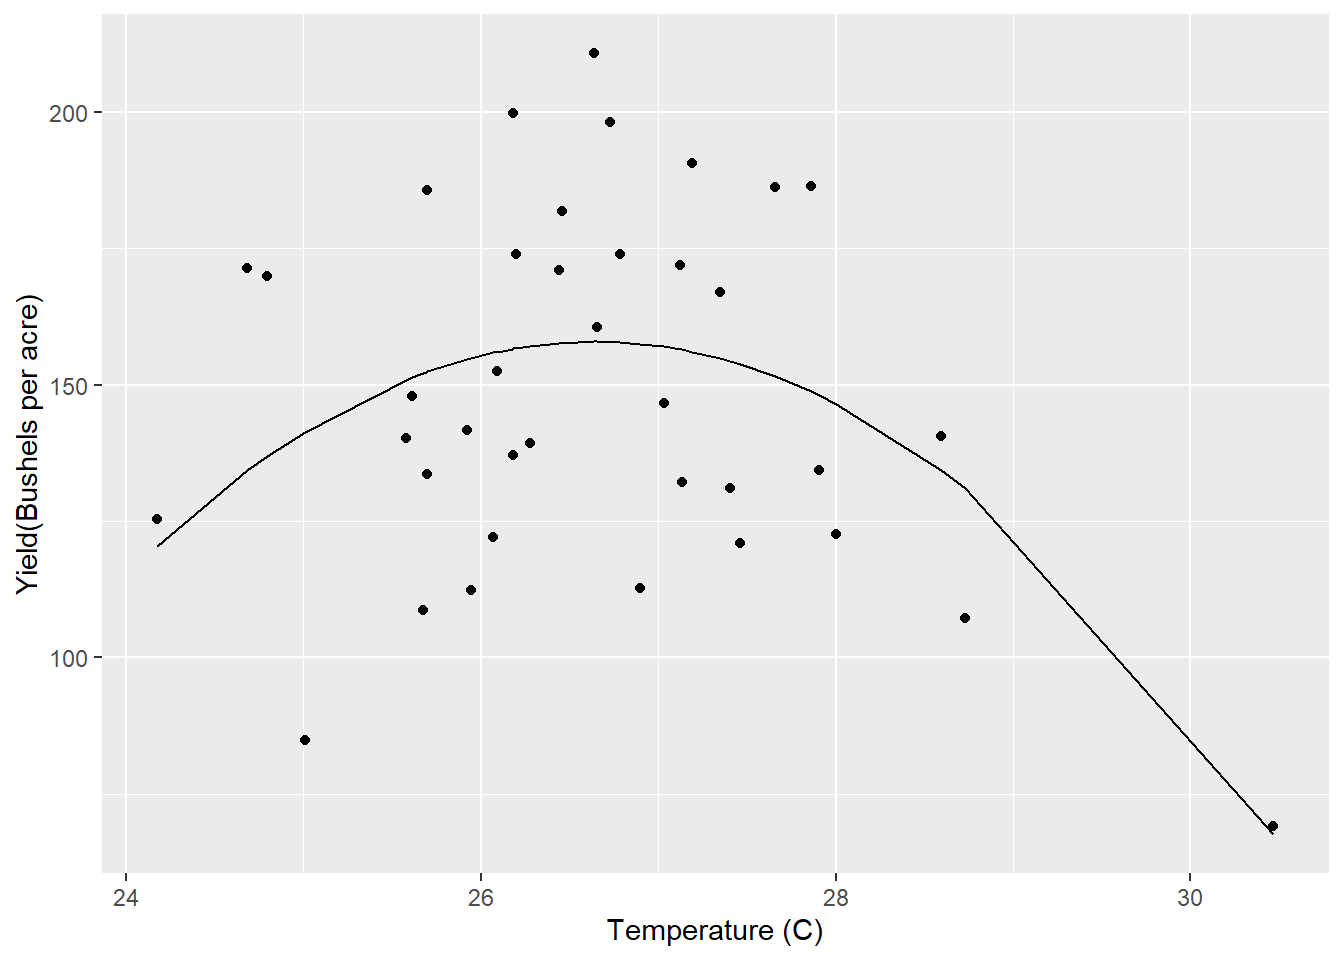
\includegraphics{bookdown-demo_files/figure-latex/unnamed-chunk-8-1.pdf}

\hypertarget{q6-write-a-function-that-makes-line-plots-of-monthly-average-temperature-at-each-site-for-a-given-year.-use-a-for-loop-to-make-these-plots-for-2005-to-2010.}{%
\subsection{Q6: Write a function that makes line plots of monthly average temperature at each site for a given year. Use a for loop to make these plots for 2005 to 2010.}\label{q6-write-a-function-that-makes-line-plots-of-monthly-average-temperature-at-each-site-for-a-given-year.-use-a-for-loop-to-make-these-plots-for-2005-to-2010.}}

Monthly average temperatures are always warmer at the Swamp Angel study plot compared to the Senator Beck study plot.This makes sense given that SASP is located in a sheltered location below treeline.SBSP is located above treeline in the alpine tundrea.

\begin{Shaded}
\begin{Highlighting}[]
\FunctionTok{names}\NormalTok{(weather\_data\_full)[}\FunctionTok{names}\NormalTok{(weather\_data\_full)}\SpecialCharTok{==}\StringTok{\textquotesingle{}air temp [K]\textquotesingle{}}\NormalTok{]}\OtherTok{\textless{}{-}}\StringTok{"air\_temp"}
\NormalTok{plotfunction}\OtherTok{\textless{}{-}}\ControlFlowTok{function}\NormalTok{(year)\{}
\NormalTok{  yeardata}\OtherTok{\textless{}{-}}\NormalTok{weather\_data\_full }\SpecialCharTok{\%\textgreater{}\%} \FunctionTok{filter}\NormalTok{(year}\SpecialCharTok{==}\NormalTok{i) }\SpecialCharTok{\%\textgreater{}\%}
    \FunctionTok{group\_by}\NormalTok{(month,site) }\SpecialCharTok{\%\textgreater{}\%}
    \FunctionTok{summarise}\NormalTok{(}\AttributeTok{mean\_temp =} \FunctionTok{mean}\NormalTok{(air\_temp,}\AttributeTok{na.rm=}\NormalTok{T))}
  \FunctionTok{print}\NormalTok{(}\FunctionTok{ggplot}\NormalTok{(yeardata,}\FunctionTok{aes}\NormalTok{(}\AttributeTok{x=}\NormalTok{month,}\AttributeTok{y=}\NormalTok{mean\_temp,}\AttributeTok{color=}\NormalTok{site))}\SpecialCharTok{+}
          \FunctionTok{geom\_line}\NormalTok{()}\SpecialCharTok{+}
          \FunctionTok{geom\_point}\NormalTok{()}\SpecialCharTok{+}
\NormalTok{          ggthemes}\SpecialCharTok{::}\FunctionTok{theme\_few}\NormalTok{()}\SpecialCharTok{+} 
          \FunctionTok{ylab}\NormalTok{(}\StringTok{"Mean Air Temperature (K)"}\NormalTok{)}\SpecialCharTok{+}
          \FunctionTok{xlab}\NormalTok{(}\StringTok{"Month"}\NormalTok{)}\SpecialCharTok{+}
\NormalTok{          ggthemes}\SpecialCharTok{::}\FunctionTok{scale\_color\_few}\NormalTok{()}\SpecialCharTok{+}
          \FunctionTok{scale\_x\_continuous}\NormalTok{(}\AttributeTok{breaks=}\FunctionTok{c}\NormalTok{(}\DecValTok{1}\NormalTok{,}\DecValTok{2}\NormalTok{,}\DecValTok{3}\NormalTok{,}\DecValTok{4}\NormalTok{,}\DecValTok{5}\NormalTok{,}\DecValTok{6}\NormalTok{,}\DecValTok{7}\NormalTok{,}\DecValTok{8}\NormalTok{,}\DecValTok{9}\NormalTok{,}\DecValTok{10}\NormalTok{,}\DecValTok{11}\NormalTok{,}\DecValTok{12}\NormalTok{))}\SpecialCharTok{+}
          \FunctionTok{ggtitle}\NormalTok{(year))}
        
\NormalTok{\}}
\ControlFlowTok{for}\NormalTok{ (i }\ControlFlowTok{in} \DecValTok{2005}\SpecialCharTok{:}\DecValTok{2010}\NormalTok{)\{}
  \FunctionTok{plotfunction}\NormalTok{(i)\}}
\end{Highlighting}
\end{Shaded}

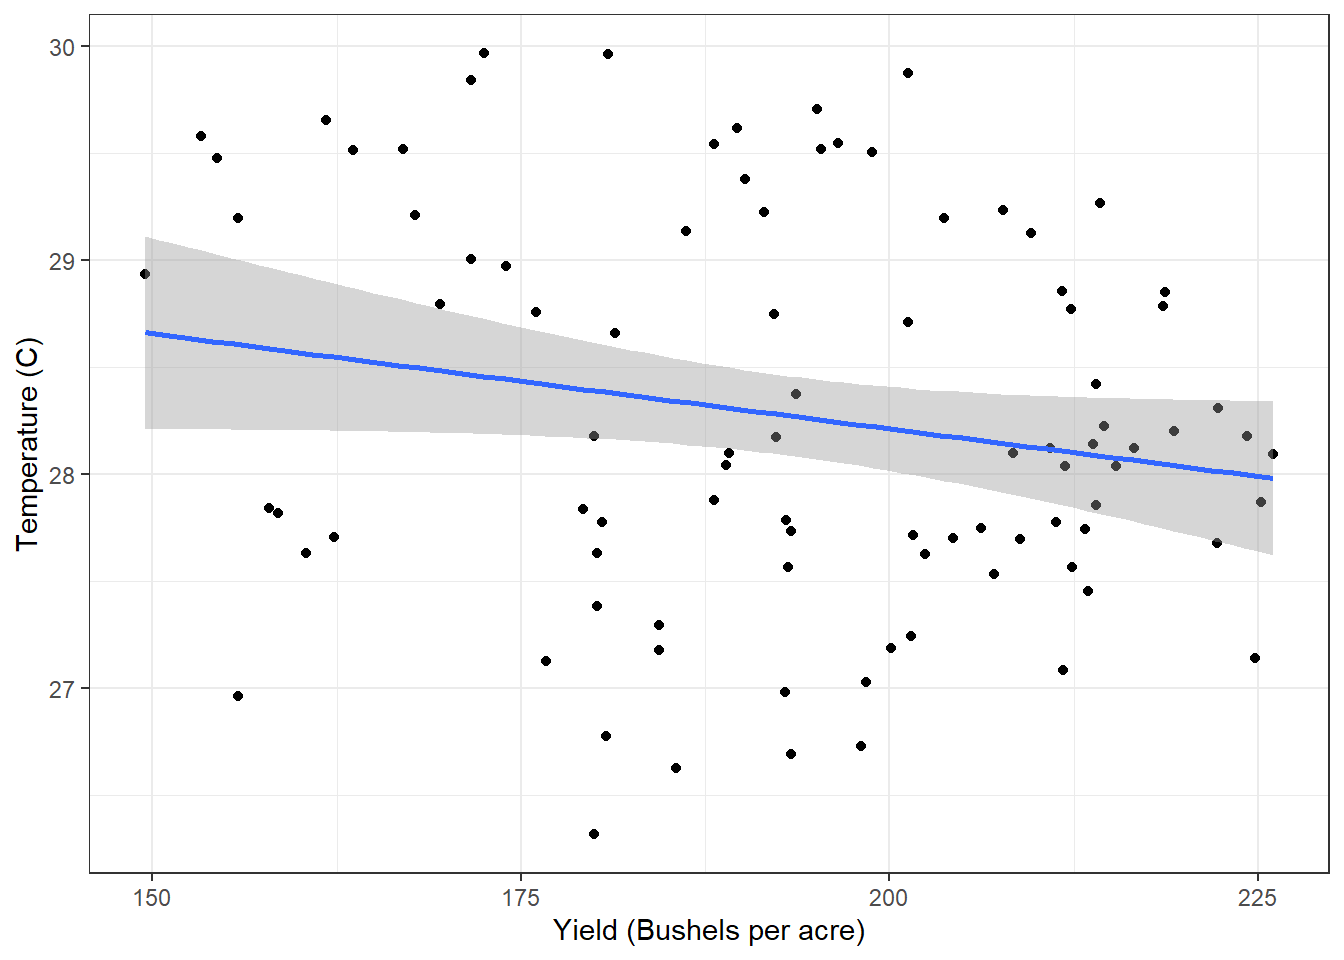
\includegraphics{bookdown-demo_files/figure-latex/unnamed-chunk-9-1.pdf} 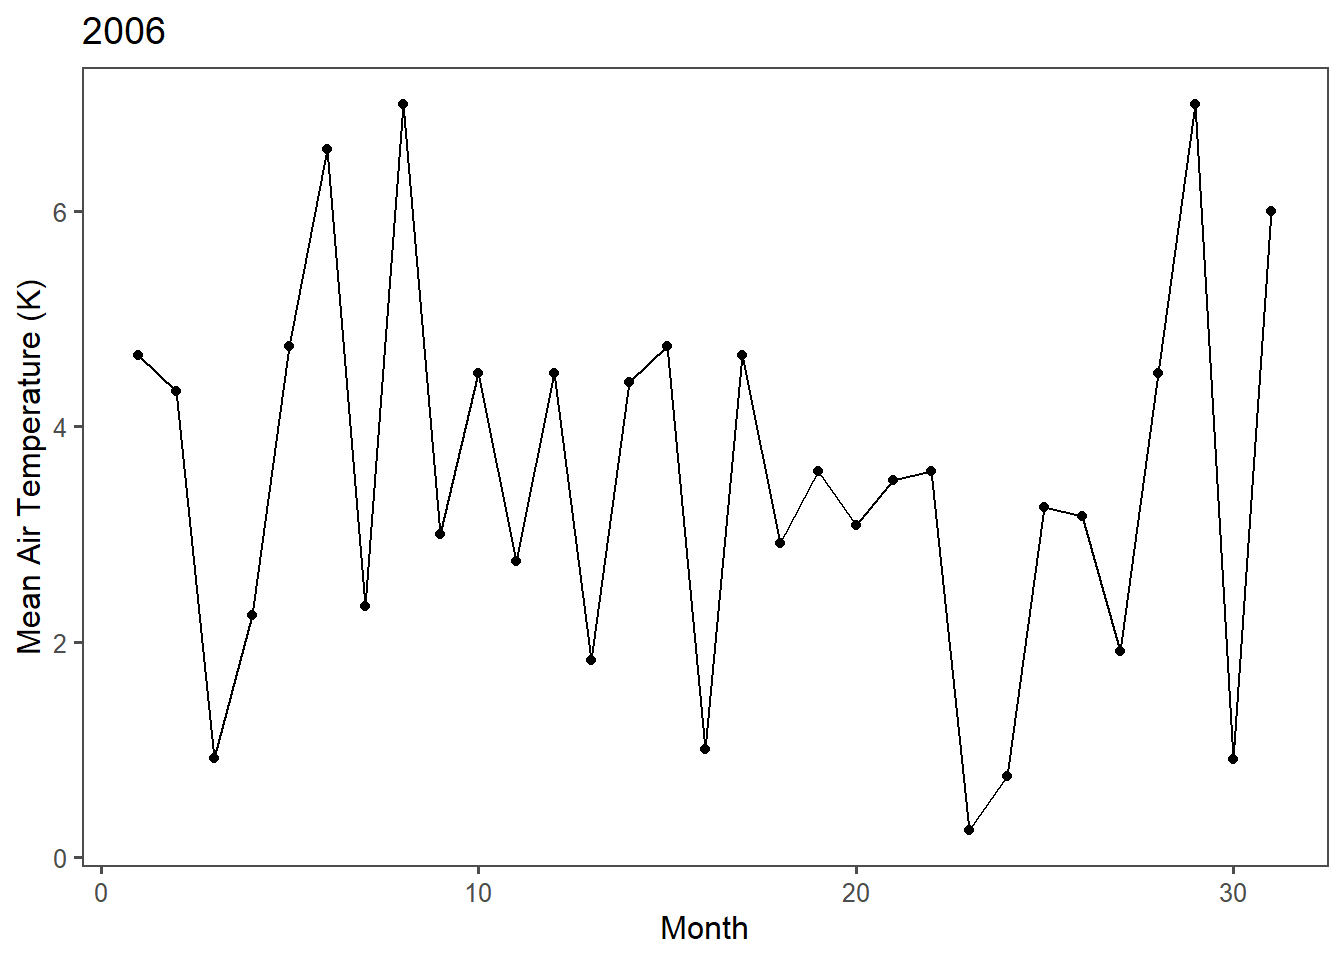
\includegraphics{bookdown-demo_files/figure-latex/unnamed-chunk-9-2.pdf} 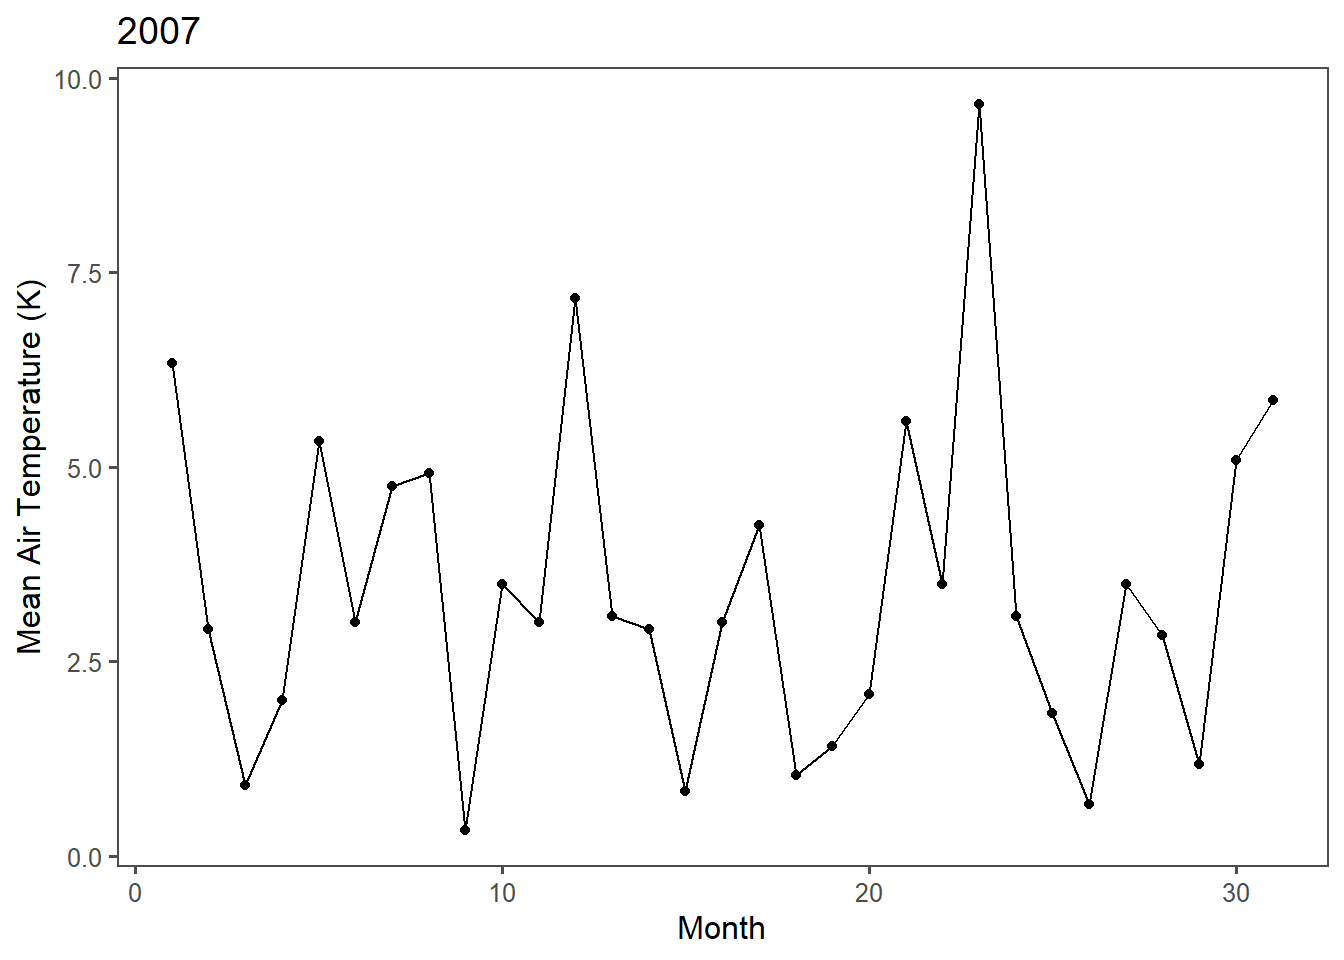
\includegraphics{bookdown-demo_files/figure-latex/unnamed-chunk-9-3.pdf} 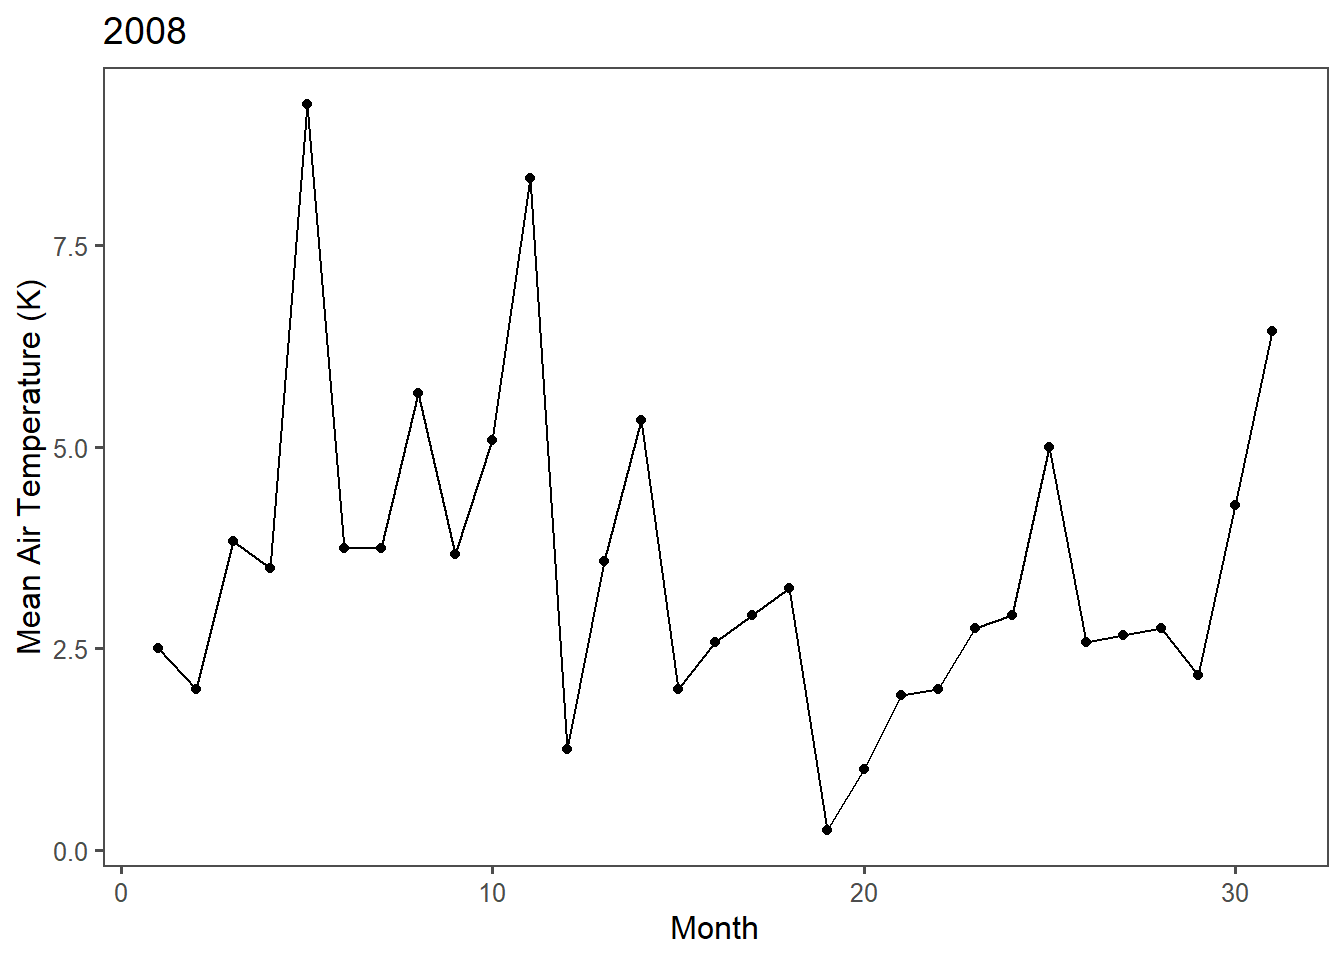
\includegraphics{bookdown-demo_files/figure-latex/unnamed-chunk-9-4.pdf} 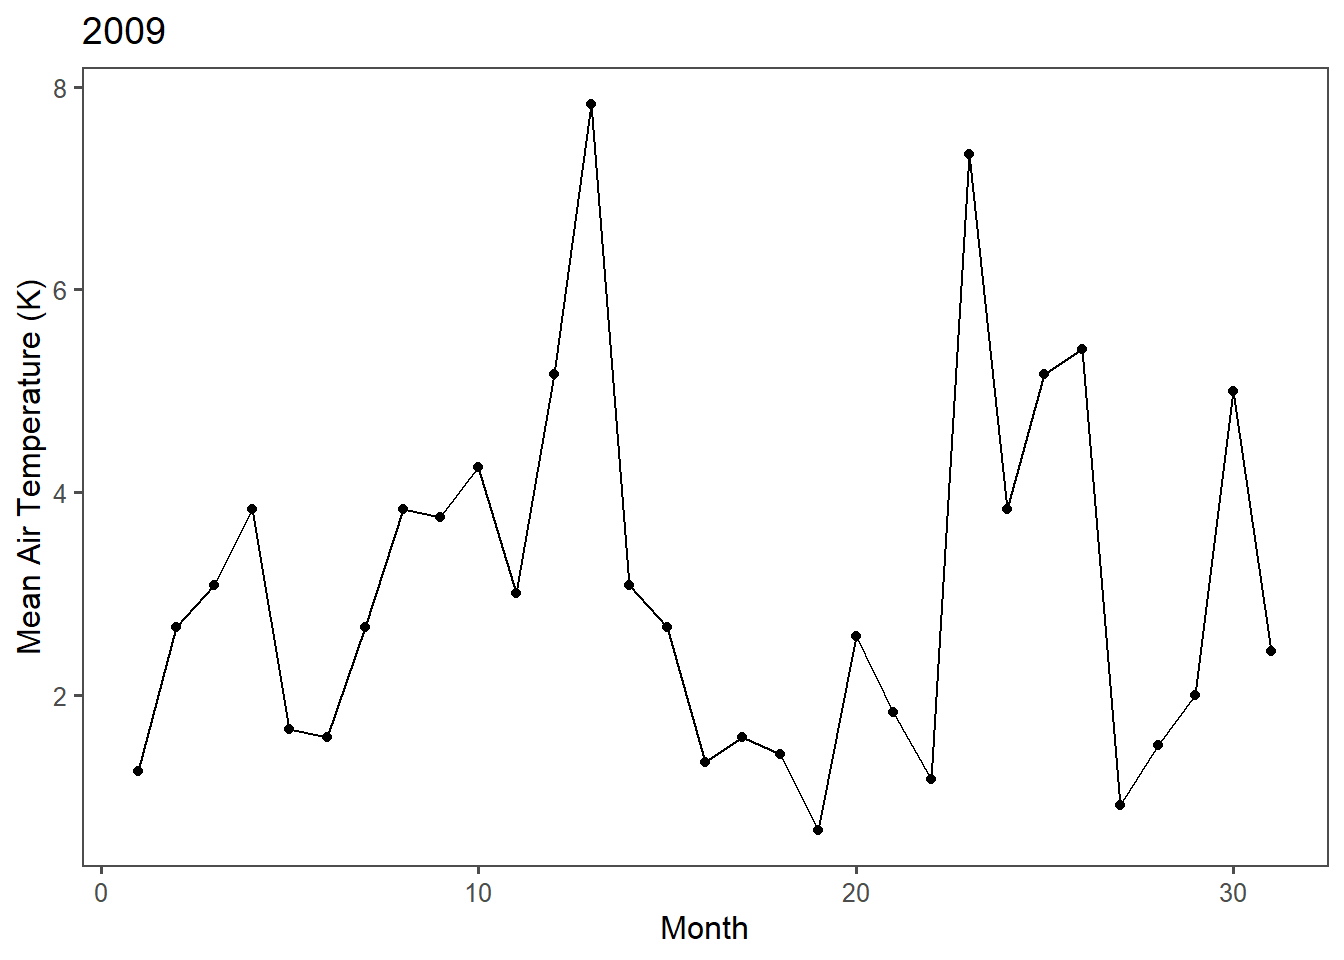
\includegraphics{bookdown-demo_files/figure-latex/unnamed-chunk-9-5.pdf} 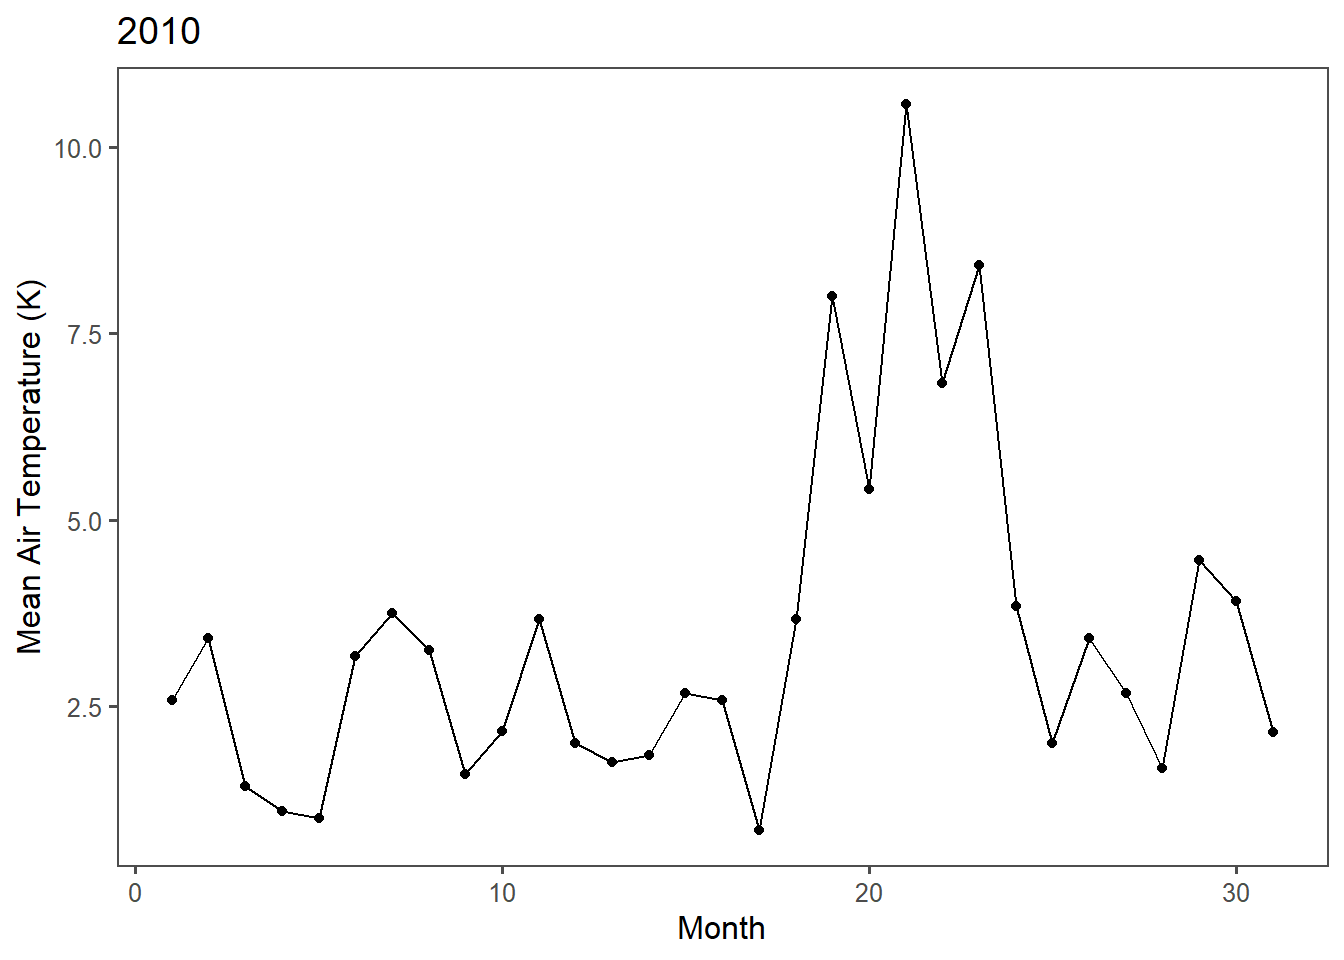
\includegraphics{bookdown-demo_files/figure-latex/unnamed-chunk-9-6.pdf}

\hypertarget{bonus-1-plot-of-average-daily-precipitation-by-day-of-year-averaged-across-all-available-years.}{%
\subsection{Bonus 1: Plot of average daily precipitation by day of year (averaged across all available years).}\label{bonus-1-plot-of-average-daily-precipitation-by-day-of-year-averaged-across-all-available-years.}}

Precipitation data here was converted from kg m-2 s-1 to mm/day. However, the precipitation values are not realistic and suggest the conversion was inaccurate. Nonetheless, the general pattern can still be gleaned from these plots.

\begin{Shaded}
\begin{Highlighting}[]
\FunctionTok{names}\NormalTok{(weather\_data\_full)[}\FunctionTok{names}\NormalTok{(weather\_data\_full)}\SpecialCharTok{==}\StringTok{\textquotesingle{}precip [kg m{-}2 s{-}1\textquotesingle{}}\NormalTok{]}\OtherTok{\textless{}{-}}\StringTok{"precip"}
\NormalTok{weather\_data\_full}\SpecialCharTok{$}\StringTok{\textasciigrave{}}\AttributeTok{precip [kg m{-}2 s{-}1]}\StringTok{\textasciigrave{}}\OtherTok{\textless{}{-}}\NormalTok{weather\_data\_full}\SpecialCharTok{$}\StringTok{\textasciigrave{}}\AttributeTok{precip [kg m{-}2 s{-}1]}\StringTok{\textasciigrave{}}\SpecialCharTok{*}\DecValTok{86400}
\NormalTok{  precip\_daily }\OtherTok{\textless{}{-}}\NormalTok{ weather\_data\_full }\SpecialCharTok{\%\textgreater{}\%} \FunctionTok{filter}\NormalTok{(year}\SpecialCharTok{==}\NormalTok{i) }\SpecialCharTok{\%\textgreater{}\%}
    \FunctionTok{group\_by}\NormalTok{(day) }\SpecialCharTok{\%\textgreater{}\%}
    \FunctionTok{summarize}\NormalTok{(}\AttributeTok{mean\_precip =} \FunctionTok{mean}\NormalTok{(}\StringTok{\textasciigrave{}}\AttributeTok{precip [kg m{-}2 s{-}1]}\StringTok{\textasciigrave{}}\NormalTok{,}\AttributeTok{na.rm=}\NormalTok{T))}
\FunctionTok{ggplot}\NormalTok{(precip\_daily,}\FunctionTok{aes}\NormalTok{(}\AttributeTok{x=}\NormalTok{day,}\AttributeTok{y=}\NormalTok{mean\_precip)) }\SpecialCharTok{+}
  \FunctionTok{geom\_point}\NormalTok{()}\SpecialCharTok{+}
  \FunctionTok{geom\_line}\NormalTok{()}\SpecialCharTok{+}
\NormalTok{  ggthemes}\SpecialCharTok{::}\FunctionTok{theme\_few}\NormalTok{()}\SpecialCharTok{+}
\NormalTok{  ggthemes}\SpecialCharTok{::}\FunctionTok{scale\_color\_few}\NormalTok{()}
\end{Highlighting}
\end{Shaded}

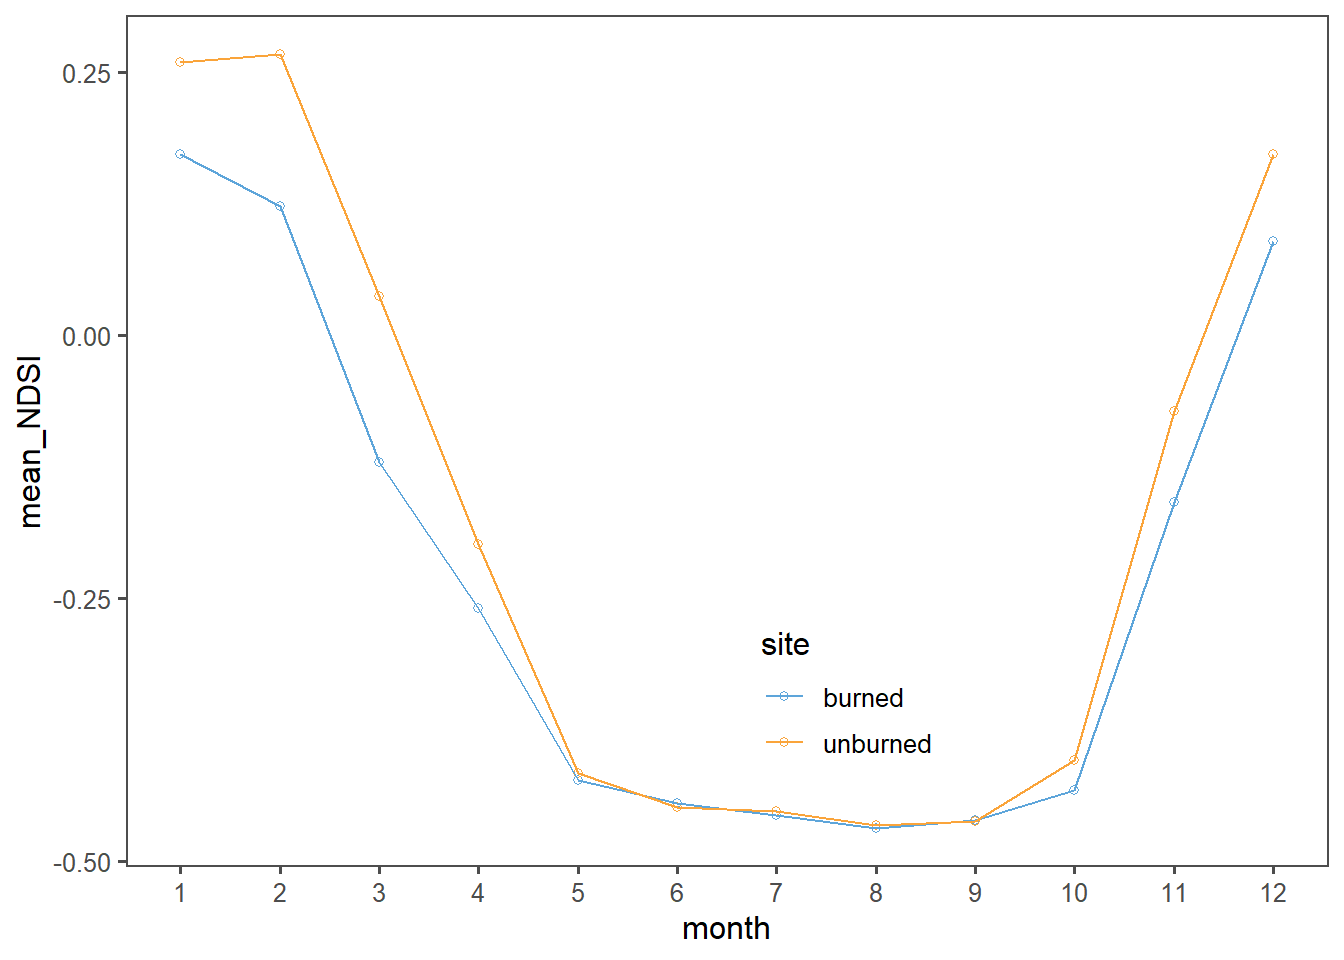
\includegraphics{bookdown-demo_files/figure-latex/unnamed-chunk-10-1.pdf}

\hypertarget{bonus-2-use-a-function-and-for-loop-to-create-yearly-plots-of-precipitation-by-day-of-year.}{%
\subsection{Bonus 2: Use a function and for loop to create yearly plots of precipitation by day of year.}\label{bonus-2-use-a-function-and-for-loop-to-create-yearly-plots-of-precipitation-by-day-of-year.}}

\begin{Shaded}
\begin{Highlighting}[]
\NormalTok{plotfunction}\OtherTok{\textless{}{-}}\ControlFlowTok{function}\NormalTok{(year)\{}
\NormalTok{  yeardata2}\OtherTok{\textless{}{-}}\NormalTok{weather\_data\_full }\SpecialCharTok{\%\textgreater{}\%} \FunctionTok{filter}\NormalTok{(year}\SpecialCharTok{==}\NormalTok{i) }\SpecialCharTok{\%\textgreater{}\%}
    \FunctionTok{group\_by}\NormalTok{(day) }\SpecialCharTok{\%\textgreater{}\%}
    \FunctionTok{summarize}\NormalTok{(}\AttributeTok{mean\_precip =} \FunctionTok{mean}\NormalTok{(}\StringTok{\textasciigrave{}}\AttributeTok{precip [kg m{-}2 s{-}1]}\StringTok{\textasciigrave{}}\NormalTok{,}\AttributeTok{na.rm=}\NormalTok{T))}
  \FunctionTok{print}\NormalTok{(}\FunctionTok{ggplot}\NormalTok{(yeardata2,}\FunctionTok{aes}\NormalTok{(}\AttributeTok{x=}\NormalTok{day,}\AttributeTok{y=}\NormalTok{mean\_precip))}\SpecialCharTok{+}
          \FunctionTok{geom\_line}\NormalTok{()}\SpecialCharTok{+}
          \FunctionTok{geom\_point}\NormalTok{()}\SpecialCharTok{+}
\NormalTok{          ggthemes}\SpecialCharTok{::}\FunctionTok{theme\_few}\NormalTok{()}\SpecialCharTok{+}
          \FunctionTok{ylab}\NormalTok{(}\StringTok{"Mean Air Temperature (K)"}\NormalTok{)}\SpecialCharTok{+}
          \FunctionTok{xlab}\NormalTok{(}\StringTok{"Month"}\NormalTok{)}\SpecialCharTok{+}
\NormalTok{          ggthemes}\SpecialCharTok{::}\FunctionTok{scale\_color\_few}\NormalTok{()}\SpecialCharTok{+}
          \FunctionTok{ggtitle}\NormalTok{(year))}
        
\NormalTok{\}}
\ControlFlowTok{for}\NormalTok{ (i }\ControlFlowTok{in} \DecValTok{2005}\SpecialCharTok{:}\DecValTok{2010}\NormalTok{)\{}
  \FunctionTok{plotfunction}\NormalTok{(i)\}}
\end{Highlighting}
\end{Shaded}

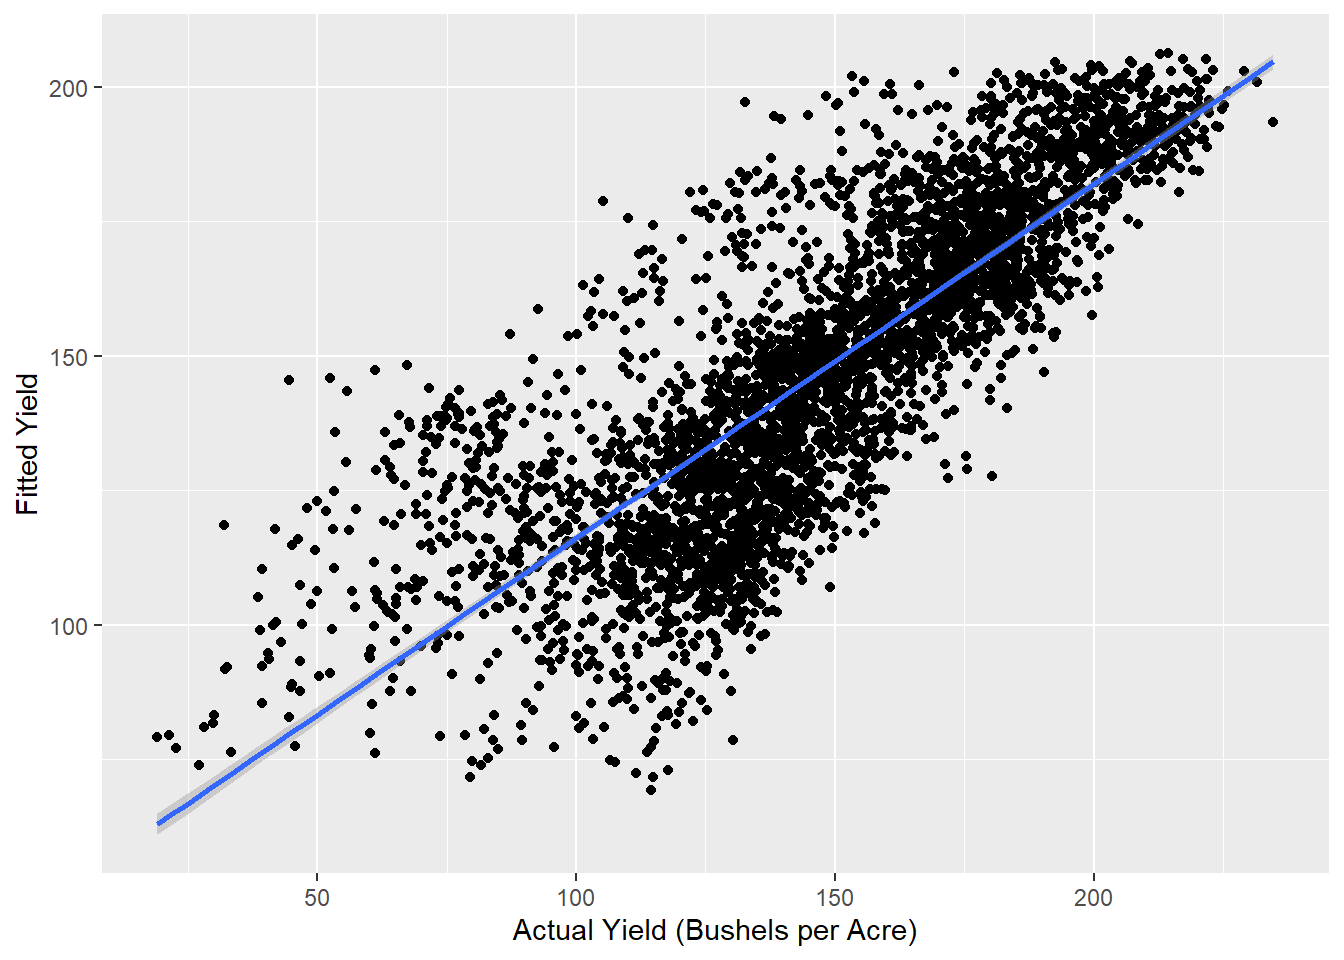
\includegraphics{bookdown-demo_files/figure-latex/unnamed-chunk-11-1.pdf} \includegraphics{bookdown-demo_files/figure-latex/unnamed-chunk-11-2.pdf} \includegraphics{bookdown-demo_files/figure-latex/unnamed-chunk-11-3.pdf} \includegraphics{bookdown-demo_files/figure-latex/unnamed-chunk-11-4.pdf} \includegraphics{bookdown-demo_files/figure-latex/unnamed-chunk-11-5.pdf} \includegraphics{bookdown-demo_files/figure-latex/unnamed-chunk-11-6.pdf}

\hypertarget{applications}{%
\chapter{Applications}\label{applications}}

Some \emph{significant} applications are demonstrated in this chapter.

\hypertarget{example-one}{%
\section{Example one}\label{example-one}}

\hypertarget{example-two}{%
\section{Example two}\label{example-two}}

\hypertarget{final-words}{%
\chapter{Final Words}\label{final-words}}

We have finished a nice book.

  \bibliography{book.bib,packages.bib}

\end{document}
